
\section{2.3 Energia Almacenada en un M.A.S}

\begin{itemize}
    \item Si no existen fuerzas de rozamiento, la energia mecanica se conserva 
\end{itemize}

\[E = K + U\]
\[= \frac{1}{2} m v^2 + \frac{1}{2} k x^2\]
\[= \frac{1}{2} k \left( \frac{m}{k} v^2 + x^2 \right)\]
\[Si: A = \sqrt{x_0^2 + \frac{\dot{x}_0^2}{\omega^2}}\]
\[A = x_0^2 + \frac{\dot{x}_0^2}{\omega^2}\]
\[\Rightarrow E = \frac{1}{2} k \left( \frac{\dot{x}_0^2}{\omega^2} + x_0^2 \right)\]
\[\boxed{E = \frac{1}{2} k A^2}\]
\begin{itemize}
    \item La energía cinética y potencial varían con el tiempo,
 sin embargo, su suma se mantiene constante.
\end{itemize}
\textbf{Energía Potencial (U) en M.A.S.}
\[U = \frac{1}{2} k x^2\]
\[U = \frac{1}{2} k \left[ A \cos(\omega t - \delta) \right]^2\]
\[\boxed{U = \frac{1}{2} k A^2 \cos^2(\omega t - \delta)}\]
\textbf{Energía Cinética (K) en M.A.S.}
\[K = \frac{1}{2} m \dot{x}^2\]
\[K = \frac{1}{2} m \left[ -A \omega \sin(\omega t - \delta) \right]^2\]
\[ = \frac{1}{2} m A^2 \omega^2 \sin^2(\omega t - \delta)\]
\[\omega^2 = \frac{k}{m}\]
\[\boxed{K = \frac{1}{2} k A^2 \sin^2(\omega t - \delta)}\]
\[E = K + U\]
\[\boxed{E = \frac{1}{2} k A^2}\]
\begin{itemize}
    \item La energia total del M.A.S es proporcional al cuadrado de su amplitud
\end{itemize}
\textbf{Propiedad General}
\begin{itemize}
    \item Graf: Energia en Funcion del Tiempo
\end{itemize}
\begin{figure}[H] % [H] fija la posición exacta (necesita el paquete float)
    \centering
    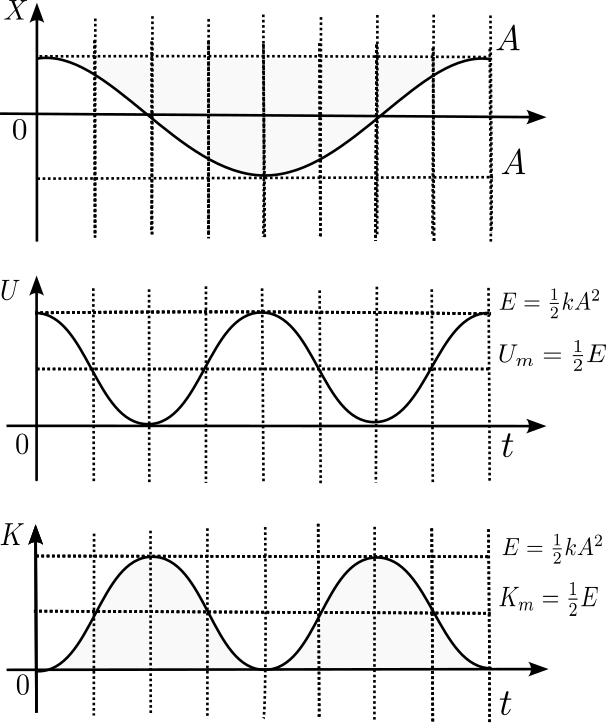
\includegraphics[width=0.4\textwidth]{img/capitulo-II/MAS.png} % ajusta el ancho
    \caption{Descripción o título de la imagen.}
    \label{fig:ejemplo} % etiqueta opcional para referencias cruzadas
\end{figure}

\begin{itemize}
    \item Graf: Energia en Funcion de la Elongacion 
\end{itemize}

\begin{figure}[H] % [H] fija la posición exacta (necesita el paquete float)
    \centering
    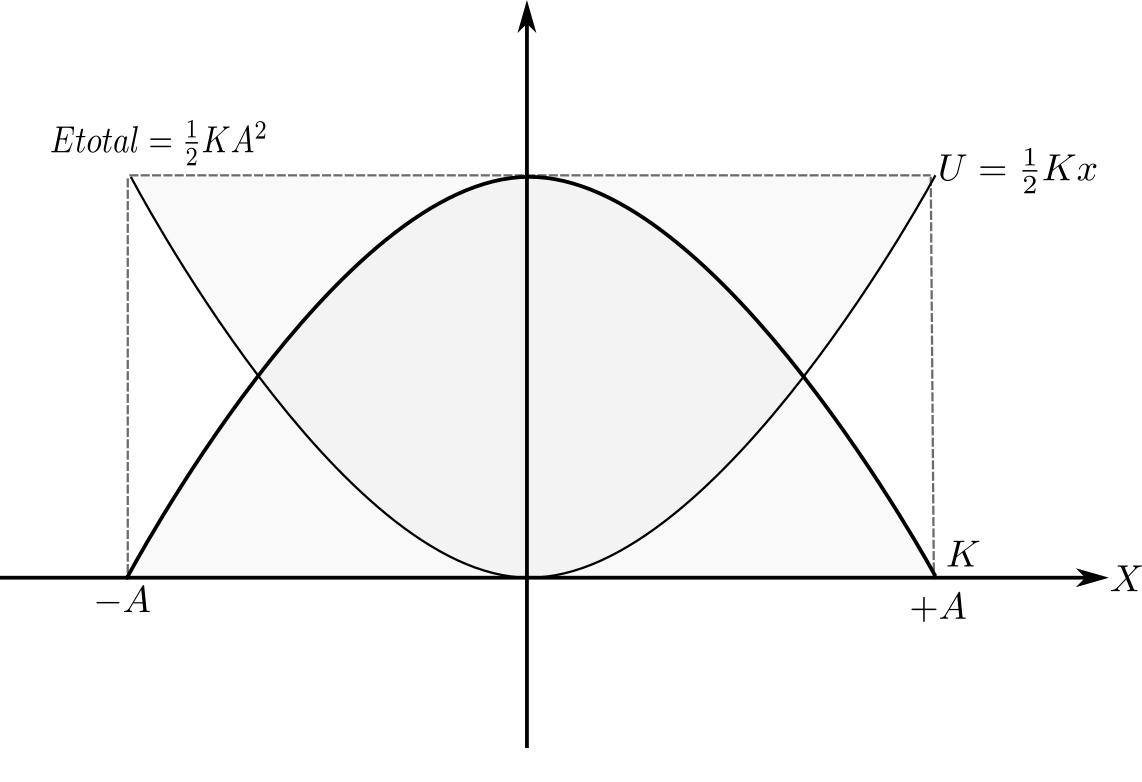
\includegraphics[width=0.5\textwidth]{img/capitulo-II/energia_en_funcion_de_la_elongacion.png} % ajusta el ancho
    \caption{Descripción o título de la imagen.}
    \label{fig:ejemplo} % etiqueta opcional para referencias cruzadas
\end{figure}

